\documentclass[10pt,conference,compsocconf]{IEEEtran}

\usepackage{hyperref}
\usepackage{graphicx}	% For figure environment


\begin{document}
\title{Title to complete... super resolution on medical images}
\author{
  Author: Marijn van der Meer\\
  Professor: Pascal Frossard, Supervisor: Mireille El Gheche \\
  \textit{Signal Processing Laboratory 4, EPFL Lausanne, Switzerland}
}

\maketitle

\begin{abstract}
\textbf{ Short description of the whole paper, to help the
  reader decide whether to read it.}

The abstract should really be written last, along with the title of
the paper. The four points that should be covered:
\begin{enumerate}
\item State the problem.
\item Say why it is an interesting problem.
\item Say what your solution achieves.
\item Say what follows from your solution.
\end{enumerate}
 \end{abstract}

\section{Introduction}\label{sec:introduction}
\textbf{Describe your problem and state your
  contributions.}
  Example of citation~\cite{jones08}
and references to another section~\ref{sec:introduction}. Example of figure and reference to Figure~\ref{fig:denoise-fourier} \begin{figure}[tbp]
  \centering
  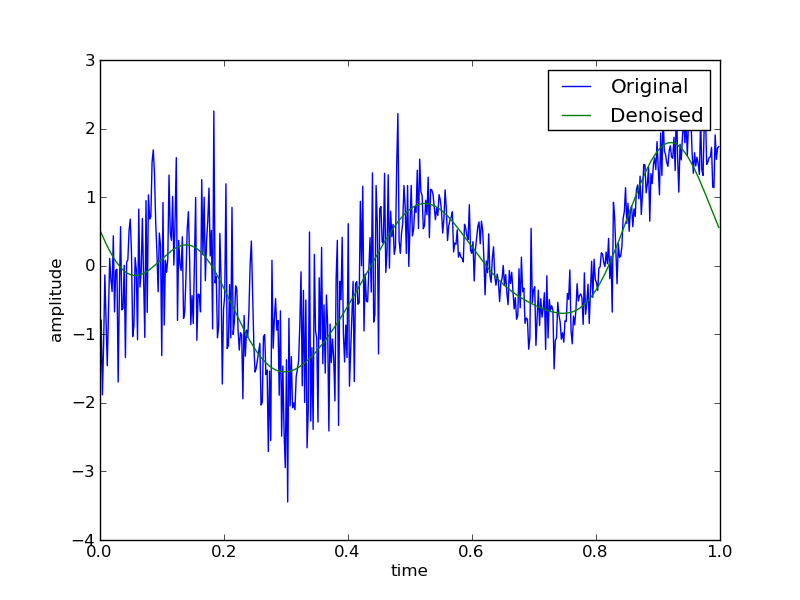
\includegraphics[width=\columnwidth]{denoised_signal_1d}
  \caption{Signal compression and denoising using the Fourier basis.}
  \vspace{-3mm}
  \label{fig:denoise-fourier}
\end{figure}

\section{State of the art}\label{sec:state-of-art}
\textbf{Survey the related work, giving credit where credit is
  due.}

\section{Models and Methods}\label{sec:models-methods}
\textbf{ Describe your idea and how it was implemented to solve
  the problem.}
The models and methods
section should describe what was
done to answer the research question, describe how it was done,
justify the experimental design, and
explain how the results were analyzed.

The model refers to the underlying mathematical model or structure which 
you use to describe your problem, or that your solution is based on. 
The methods on the other hand, are the algorithms used to solve the problem. 
In some cases, the suggested method directly solves the problem, without having it 
stated in terms of an underlying model. Generally though it is a better practice to have 
the model figured out and stated clearly, rather than presenting a method without specifying 
the model. In this case, the method can be more easily evaluated in the task of fitting 
the given data to the underlying model.

The methods part of this section, is not a step-by-step, directive,
protocol as you might see in your lab manual, but detailed enough such
that an interested reader can reproduce your
work~\cite{anderson04,wavelab}.

The methods section of a research paper provides the information by
which a study's validity is judged.
Therefore, it requires a clear and precise description of how an
experiment was done, and the rationale
for why specific experimental procedures were chosen.
It is usually helpful to
structure the methods section by~\cite{kallet04methods}:
\begin{enumerate}
\item Layout the model you used to describe the problem or the solution.
\item Describing the algorithms used in the study, briefly including
  details such as hyperparameter values (e.g. thresholds), and
  preprocessing steps (e.g. normalizing the data to have mean value of
  zero).
\item Explaining how the materials were prepared, for example the
  images used and their resolution.
\item Describing the research protocol, for example which examples
  were used for estimating the parameters (training) and which were
  used for computing performance.
\item Explaining how measurements were made and what
  calculations were performed. Do not reproduce the full source code in
  the paper, but explain the key steps.
\end{enumerate}
 

\section{Results}\label{sec:results}
\textbf{Show evidence to support your claims made in the
  introduction.}
  Organize the results section based on the sequence of table and
figures you include. Prepare the tables and figures as soon as all
the data are analyzed and arrange them in the sequence that best
presents your findings in a logical way. A good strategy is to note,
on a draft of each table or figure, the one or two key results you
want to address in the text portion of the results.

\section{Discussion}\label{sec:discussion}
  \textbf{Discuss the strengths and weaknesses of your
  approach, based on the results. Point out the implications of your
  novel idea on the application concerned.}
  
\section{Summary}\label{sec:summary}
  \textbf{Summarise your contributions in light of the new
  results.}

\section*{Acknowledgements}
TO COMPLETE.

\newpage
\bibliographystyle{IEEEtran}
\bibliography{literature}

\end{document}